\documentclass{article}
\usepackage{amsmath}
\usepackage{graphicx}
\usepackage{fancyhdr}
\usepackage[sorting=none]{biblatex}
\usepackage[margin=1in]{geometry}
\usepackage{listings}
\usepackage[hidelinks]{hyperref}
\usepackage{subfigure}
\usepackage{float}
\hypersetup{
    colorlinks=true,
    linkcolor=teal,
    filecolor=magenta,      
    urlcolor=teal,
    citecolor = teal
    }
\usepackage{xcolor}
\usepackage{xepersian}
\setlength\headheight{28pt} 
\addbibresource{bibliography.bib}
\settextfont[Path={./font/}, Scale=1.3]{IRLotus}
\setlatintextfont[Scale=1]{Times New Roman}
\renewcommand{\baselinestretch}{1.5}
\pagestyle{fancy}
\fancyhf{}
\rhead{
\includegraphics[width=1cm]{img/Logo.png}پروژه اول  }
\lhead{\thepage}
 \rfoot{علیرضا امیری}
\lfoot{ایمان گندمی}
\renewcommand{\headrulewidth}{1pt}
\renewcommand{\footrulewidth}{1pt}
\AtBeginDocument{
	\def\chapterautorefname{فصل}%
	\def\sectionautorefname{پاسخ سوال}%
	\def\subsectionautorefname{بخش}%
	\def\subsubsectionautorefname{بخش}%
	\def\equationautorefname{رابطهٔ}%
    \def\lstlistingautorefname{برنامۀ}%
}
\renewcommand{\lstlistingname}{Code}

\definecolor{codegreen}{rgb}{0,0.6,0}
\definecolor{codegray}{rgb}{0.5,0.5,0.5}
\definecolor{codepurple}{rgb}{0.58,0,0.82}
\definecolor{backcolour}{rgb}{0.95,0.95,0.92}

\lstdefinestyle{mystyle}{
	backgroundcolor=\color{backcolour},   
	commentstyle=\color{codegreen},
	keywordstyle=\color{magenta},
	numberstyle=\tiny\color{codegray},
	stringstyle=\color{codepurple},
	basicstyle=\ttfamily\footnotesize,
	breakatwhitespace=false,         
	breaklines=true,                 
	captionpos=b,                    
	keepspaces=true,                 
	numbers=left,                    
	numbersep=5pt,                  
	showspaces=false,                
	showstringspaces=false,
	showtabs=false,                  
	tabsize=2
}

\lstset{style=mystyle}

\begin{document}

\begin{titlepage}
\begin{center}
\defpersianfont\nast[Path={./font/}, Scale=2]{IranNastaliq}
\centerline{{
\includegraphics[width=5cm]{img/Logo.png}}}
\centerline{\textcolor[rgb]{0,0,0.5}{\nast \large  دانشگاه صنعتی خواجه نصیرالدین طوسی}}
\centerline{\textcolor[rgb]{0,0,0.5}{\nast \bfseries دانشکدۀ مهندسی برق - گروه مهندسی کنترل}}

\vfill
        
\Huge
\textbf{رباتیک}\\
\textbf{پاسخ پروژه اول}\\
        
\vfill
        
\begin{table}[ht]
    \centering
    \huge
    \begin{tabular}{|c|c|}
    \hline
    نام و نام خانوادگی &  ایمان گندمی\\
    \hline
    شمارۀ دانشجویی &40223704\\
    \hline
    نام و نام خانوادگی &   علیرضا امیری\\
    \hline
    شمارۀ دانشجویی &40202414\\
    \hline
    تاریخ & آبان‌ماه 1403\\
    \hline
    \end{tabular}
\end{table}
\end{center}
\end{titlepage}


\tableofcontents \clearpage
\listoffigures \clearpage
%\listoftables \clearpage
%\lstlistoflistings \clearpage
\newpage

\section{سوال اول - مشخصات فنی ربات}\label{Section1}

برای به دست آوردن مشخصات فنی ربات مورد استفاده در این پژوهش، با مراجعه به دیتاشیت ربات IRB 760، می‌توان اطلاعات لازم از جمله ابعاد، محدودیت‌های کاری مفاصل، فضای کاری، توان مصرفی، دمای کاری و سایر مشخصات مهم را استخراج کرد. این ربات چهار محوره با ظرفیت بار ۴۵۰ کیلوگرم و دسترسی ۳.۱۸ متر، برای کاربردهایی مانند پالت‌گذاری، دپالت‌گذاری، جابجایی مواد و پرس‌کاری طراحی شده است. ربات IRB 760 با کنترلر OmniCore و نرم‌افزارهای QuickMove™ و TrueMove™، حرکات نرم و دقیقی را ارائه می‌دهد که برای جابجایی محصولات حساس نیز مناسب است.

این ربات دارای چهار محور است که به ترتیب در بازه‌های ±۱۸۰ درجه (محور اول)، +۸۵ تا -۴۲ درجه (محور دوم)، +۱۲۰ تا -۲۰ درجه (محور سوم) و ±۳۰۰ درجه (محور چهارم) حرکت می‌کنند و حداکثر سرعت محور چهارم به ۱۶۰ درجه بر ثانیه می‌رسد. دقت تکرارپذیری آن ۰.۰۵ میلی‌متر و استاندارد حفاظت IP67 را داراست که آن را برای محیط‌های گردوغبار و مرطوب مناسب می‌سازد. محدوده دمای کاری ربات بین ۰ تا ۵۰ درجه سانتی‌گراد است و برای دوره‌های کوتاه‌مدت تا ۷۰ درجه را نیز تحمل می‌کند. با مصرف برق ۲.۷۵ کیلووات و وزن ۲۳۱۰ کیلوگرم، این ربات می‌تواند تا ۸۸۰ چرخه در ساعت با بار کامل انجام دهد که برای کاربردهای سنگین صنعتی، به‌ویژه در خودروسازی، گزینه‌ای مناسب به شمار می‌رود.

\begin{figure}[H]
    \centering
    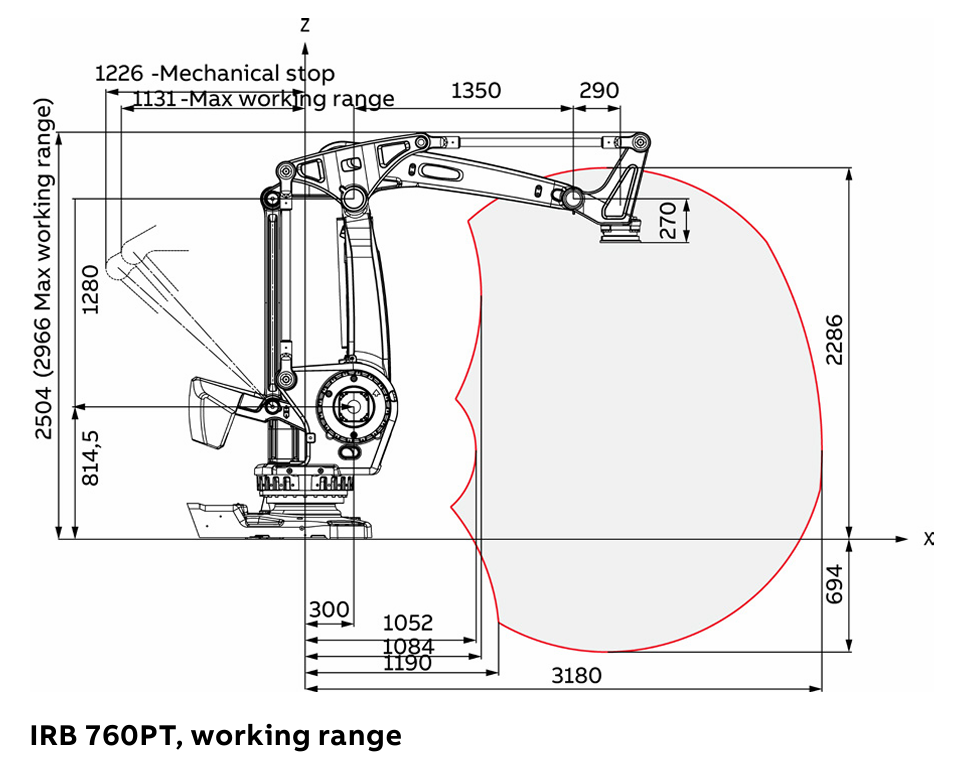
\includegraphics[width=0.75\linewidth]{Working_Range.png}
    \caption{فضای کاری ربات}
    \label{fig:enter-label}
\end{figure}
\begin{figure}[H]
    \centering
    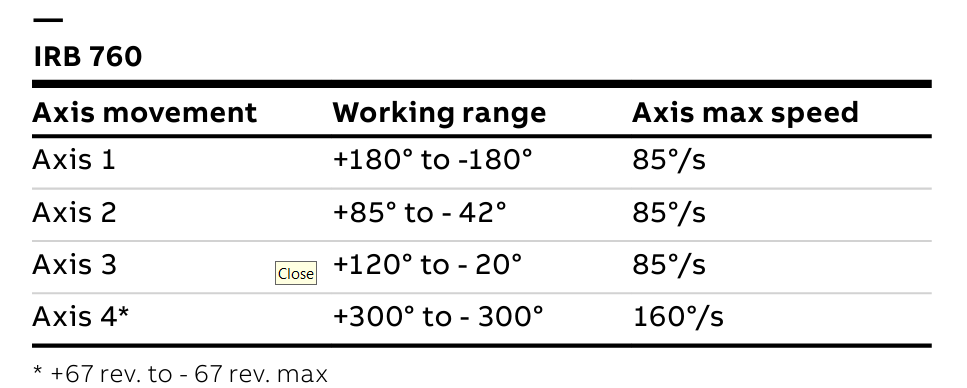
\includegraphics[width=0.5\linewidth]{Links_Working_Rangepng.png}
    \caption{محدودیت های مفاصل ربات}
    \label{fig:enter-label}
\end{figure}

\section{سوال دوم - روش دناویت-هارتنبرگ}\label{Section2}
برای حل مسئله‌ی سینماتیک مستقیم به روش دناویت-هارتنبرگ، ابتدا پارامترهای ماتریس DH باید مشخص شوند.
برای این منظور ماتریس های تبدیل را با استفاده از تابع تعریف شده چنین به دست می‌آوریم:

\[
\begin{aligned}
    T_1 &= \text{DH}(0, \frac{\pi}{2}, 0, \theta_1) \\
    T_2 &= \text{DH}(l_1, 0, 0, \theta_2) \\
    T_3 &= \text{DH}(l_5, 0, 0, \theta_3)
\end{aligned}
\]

ماتریس تبدیل این جابه‌جایی از ضرب ماتریس‌های بالا به دست می‌آید. با جداسازی ماتریس دوران و انتقال از این ماتریس تبدیل در نهایت خواهیم داشت:

\[
P_{\text{DH}} = 
\begin{pmatrix}
1.0 \cos \left(\theta_1 \right) \left(l_5 \cos \left(\theta_2 + \theta_3 \right) + l_1 \cos \left(\theta_2 \right)\right) \\
1.0 \sin \left(\theta_1 \right) \left(l_5 \cos \left(\theta_2 + \theta_3 \right) + l_1 \cos \left(\theta_2 \right)\right) \\
1.0 l_5 \sin \left(\theta_2 + \theta_3 \right) + 1.0 l_1 \sin \left(\theta_2 \right)
\end{pmatrix}
\]

\[
R_{\text{DH}} = 
\begin{pmatrix}
1.0 \cos \left(\theta_2 + \theta_3 \right) \cos \left(\theta_1 \right) & -1.0 \sin \left(\theta_2 + \theta_3 \right) \cos \left(\theta_1 \right) & 1.0 \sin \left(\theta_1 \right) \\
1.0 \cos \left(\theta_2 + \theta_3 \right) \sin \left(\theta_1 \right) & -1.0 \sin \left(\theta_2 + \theta_3 \right) \sin \left(\theta_1 \right) & -1.0 \cos \left(\theta_1 \right) \\
1.0 \sin \left(\theta_2 + \theta_3 \right) & 1.0 \cos \left(\theta_2 + \theta_3 \right) & 0
\end{pmatrix}
\]

\section{سوال سوم - روش پیچه}\label{Section3}
حل مسئله ی سینماتیک مستقیم این ربات، نیازمند مشخص کردن محورهای پیچه می‌باشد. در ادامه، با استفاده از موقعیت و جهت بردارها، می‌توان پارامترهای پیچه را استخراج کرد.
با در نظر گرفتن ساختار این ربات، ماتریس های تبدیل در هر مفصل به صورت زیر به دست می آیند:
\[
S_1 = SR(0, 0, 1, 0, 0, 0, \theta_1, 0);
\]
\[
S_2 = SR(0, -1, 0, 0, 0, 0, \theta_2, 0);
\]
\[
S_3 = SR(0, -1, 0, l_1, 0, 0, \theta_3, 0);
\]

حاصل ضرب این ماتریس ها به طور مستقیم، ماتریس تبدیل نهایی را به وجود نمی آورد و نیاز است در گام بعد، ماتریس دوران و انتقال بین مختصات مرجع و مختصات پنجه ی ربات نیز لحاظ شود. در این قسمت، حاصل ضرب ماتریس‌های تبدیل بالا چنین به دست می آیند:

\[
S = S_1 \cdot S_2 \cdot S_3 = 
\begin{array}{l}
\begin{pmatrix}
\cos \left(\theta_2 + \theta_3 \right) \cos \left(\theta_1 \right) & -\sin \left(\theta_1 \right) & -\sin \left(\theta_2 + \theta_3 \right) \cos \left(\theta_1 \right) & -l_1 \cos \left(\theta_1 \right) \sigma_1 \\
\cos \left(\theta_2 + \theta_3 \right) \sin \left(\theta_1 \right) & \cos \left(\theta_1 \right) & -\sin \left(\theta_2 + \theta_3 \right) \sin \left(\theta_1 \right) & -l_1 \sin \left(\theta_1 \right) \sigma_1 \\
\sin \left(\theta_2 + \theta_3 \right) & 0 & \cos \left(\theta_2 + \theta_3 \right) & -l_1 \left(\sin \left(\theta_2 + \theta_3 \right) - \sin \left(\theta_2 \right)\right) \\
0 & 0 & 0 & 1
\end{pmatrix}
\\
\\
\text{where}
\\
\\
\;\; \sigma_1 = \cos \left(\theta_2 + \theta_3 \right) - \cos \left(\theta_2 \right)
\end{array}
\]

حال برای تعریف ماتریس تبدیل از دستگاه مختصات مرجع به مبدا خواهیم داشت:
\[
S_{\text{O}} = 
\begin{pmatrix}
1 & 0 & 0 & l_1 + l_5 \\
0 & 0 & -1 & 0 \\
0 & 1 & 0 & 0 \\
0 & 0 & 0 & 1
\end{pmatrix}
\]

در نهایت، ماتریس تبدیل برای این ربات از ضرب ماتریس S
در ماتریس تبدیل دستگاه های مختصات مرجع و مبدا به محاسبه می شود. پس از جداسازی ماتریس دوران و انتقال این ماتریس تبدیل خواهیم داشت:
\[
P_{\text{S}} = 
\begin{pmatrix}
\cos \left(\theta_1 \right) \left(l_5 \cos \left(\theta_2 + \theta_3 \right) + l_1 \cos \left(\theta_2 \right)\right) \\
\sin \left(\theta_1 \right) \left(l_5 \cos \left(\theta_2 + \theta_3 \right) + l_1 \cos \left(\theta_2 \right)\right) \\
l_5 \sin \left(\theta_2 + \theta_3 \right) + l_1 \sin \left(\theta_2 \right)
\end{pmatrix}
\]
\[
R_{\text{S}} = 
\begin{pmatrix}
\cos \left(\theta_2 + \theta_3 \right) \cos \left(\theta_1 \right) & -\sin \left(\theta_2 + \theta_3 \right) \cos \left(\theta_1 \right) & \sin \left(\theta_1 \right) \\
\cos \left(\theta_2 + \theta_3 \right) \sin \left(\theta_1 \right) & -\sin \left(\theta_2 + \theta_3 \right) \sin \left(\theta_1 \right) & -\cos \left(\theta_1 \right) \\
\sin \left(\theta_2 + \theta_3 \right) & \cos \left(\theta_2 + \theta_3 \right) & 0
\end{pmatrix}
\]

در نهایت، از مقایسه ی ماتریس های تبدیل به دست آمده از دو روش دناویت هارتنبرگ و پیچه، می توانیم صحت محاسبات انجام شده را به دست آوریم. برای این منظور، با محاسبه ی تفاضل ماتریس های به دست آمده از هر این دو روش خواهیم داشت:
\[
\text{Error} = T_{\text{DH}} - T_{\text{S}} = 
\begin{pmatrix}
0 & 0 & 0 & 0 \\
0 & 0 & 0 & 0 \\
0 & 0 & 0 & 0 \\
0 & 0 & 0 & 0
\end{pmatrix}
\]

در نتیجه، صحت جواب های به دست آمده از این دو روش اثبات می شوند.

\section{سوال چهارم - سینماتیک وارون}\label{Section4}

در این بخش، با محاسبه ی روابط هندسی حاکم بر فضای سه بعدی، با دریافت ورودی های موقعیت ابزار و با معین بودن اندازه ی لینک ها خواهیم داشت:

\begin{align*}
    \theta_1 &= \arctan\left(\frac{y}{x}\right) \\
    r &= \sqrt{x^2 + y^2} \\
    d &= \sqrt{r^2 + z^2} \\
    \theta_3 &= \arccos\left(\frac{d^2 - l_1^2 - l_5^2}{2 \cdot l_1 \cdot l_5}\right) \\
    \text{Total angle} &= \arctan\left(\frac{z}{r}\right) \\
    \theta_2 &= \text{Total angle} - \theta_3
\end{align*}

با استفاده از روابط بالا، می توان زوایای مفصلی متناظر با هر موقعیت ابزار را به دست آورد.

\section{سوال پنجم - صحت سنجی با SolidWorks}\label{Section3}

در این بخش، ابتدا با جایگذاری مقادیر عددی داده شده مطابق با داده های سوال و محاسبه ی موقعیت ابزار ربات به وسیله ی ماتریس های تبدیل به دست آمده از دو روش دناویت هارتنبرگ و یا پیچه، پاسخی را به دست می آوریم. در ادامه با طراحی هندسی ربات و تنظیم زوایای آن، مختصات نقطه ی ابزار را اندازه می گیریم.

\subsection{محاسبه ی عددی}
پیش از آنکه مقادیر زاویه ها را در ماتریس های تبدیل قرار دهیم، لازم است ابتدا زوایای موجود در فایل طراحی ربات به زوایای مورد استفاده در ماتریس تبدیل تغییر کنند. 
برای این منظور، مقادیر \(\theta_1^*, \; \theta_2^*, \; \theta_3^*\)
که زوایای داده شده در فایل طراحی هستند با رابطه ی زیر تبدیل به روابط مورد استفاده در ماتریس تبدیل می شوند:
\[
\theta_1 = \theta_1^*, \quad \theta_2 = \theta_3^*, \quad \theta_3 = \pi - \theta_3^* + \theta_2^*
\]

با جایگذاری مقادیر داده شده در این رابطه خواهیم داشت:
\[
\theta_1^* = 0, \quad \theta_2^* = \frac{\pi}{4}, \quad \theta_3^* = \frac{3\pi}{4}
\implies
\theta_1 = 0, \quad \theta_2 = \frac{3\pi}{4}, \quad \theta_3 = \frac{\pi}{4}
\]
با استفاده از این مقادیر و محاسبه ی ماتریس تبدیل و حل مسئله ی سینماتیک مستقیم، موقعیت و جهت گیری نهایی ابزار به صورت زیر به دست می آید:
\[
P_{\text{end-effector}} =
\begin{pmatrix}
-1.8597 \\
0 \\
-0.0495
\end{pmatrix}
\]

\[
R_{\text{end-effector}} =
\begin{pmatrix}
-0.7071 & 0.7071 & 0 \\
0 & 0 & -1.0000 \\
-0.7071 & -0.7071 & 0
\end{pmatrix}
\]

\subsection{محاسبه ی هندسی}
در این روش، با رسم طرح ساده شده ی ربات و تنظیم اندازه‌ی لینک‌ها، محدودیت های اعمال شده بر آن و همچنین تنظیم زوایا بر اساس مقادیر داده شده، موقعیت نهایی ابزار را به دست می آوریم. 

\begin{figure}[H]
    \centering
    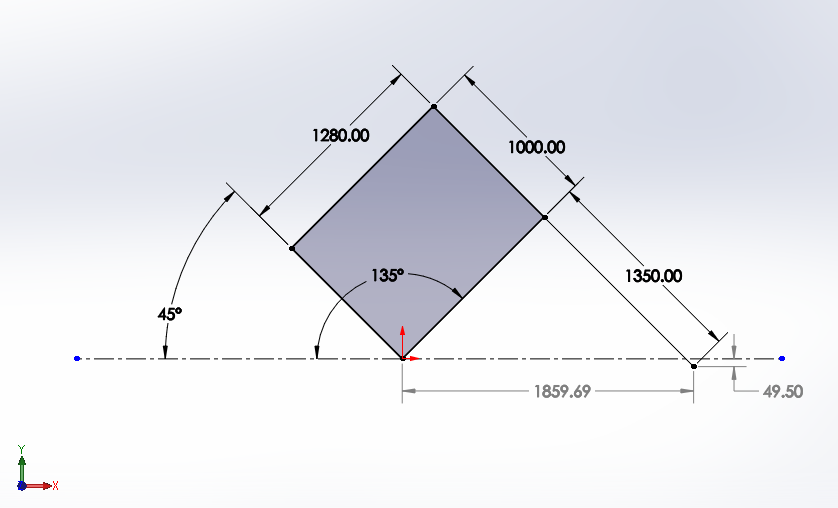
\includegraphics[width=1\linewidth]{solid_sketch.PNG}
    \caption{طرح رسم شده از ربات}
    \label{fig:Robot_cad}
\end{figure}

\textbf{
مشاهده می شود که موقعیت به دست آمده برای ابزار ربات در این روش، با موقعیت محاسبه شده به وسیله ی کد مطابقت دارد.}

\section{سوال ششم -شبیه سازی}\label{Section6}
برای شبیه سازی عملکرد ربات مورد استفاده در این پژوهش، ساختار ربات به نرم افزار SimScape وارد شده است.

\begin{figure}[H]
    \centering
    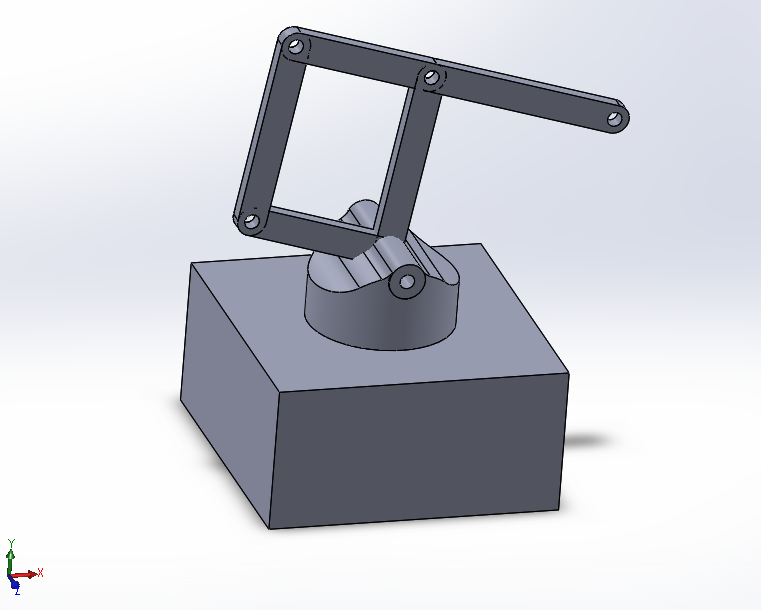
\includegraphics[width=0.5\linewidth]{robot_solid.PNG}
    \caption{طرح ربات در سالیدورکس}
    \label{fig:enter-label}
\end{figure}

\begin{figure}[H]
    \centering
    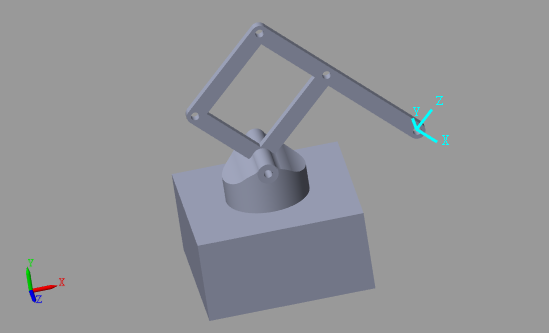
\includegraphics[width=0.5\linewidth]{robot_simscape.PNG}
    \caption{طرح ربات در SimScape}
    \label{fig:enter-label}
\end{figure}

پس از وارد کردن طراحی ربات به این نرم افزار، ساختار کلی مفاصل آن توسط سیمولینک ساخته می شود. 
برای اعمال ورودی های مختلف به این دستگاه و اندازه گیری موقعیت ابزار، لازم است بلوک های دیگری نیز به آن اضافه شوند که در ادامه به توضیح هر یک خواهیم پرداخت.
برای اعمال ورودی زوایای مناسب به ربات، لازم است تغییراتی بر آن اعمال شود. در گام اول، برای یکسان سازی زاوبه‌ی 0 هر یک از محورهای دوران، با مقایسه ی طرح داده شده ی ربات و نتایج شبیه سازی، تغییرات زاوبه برای هر یک از محور های دوران به دست آمد. تغییر زوایا با اضافه کردن مقدار ثابتی به هر یک از محورهای دوران صورت می گیرد. 
در شکل \ref{fig:Robot_Input} این بلوک ها نمایش داده شده اند.
در نهایت، با ضرب مقدار عددی ثابت، واحد زوایای وارد شده به رادیان تبدیل می شود.

\begin{figure}[h]
    \centering
    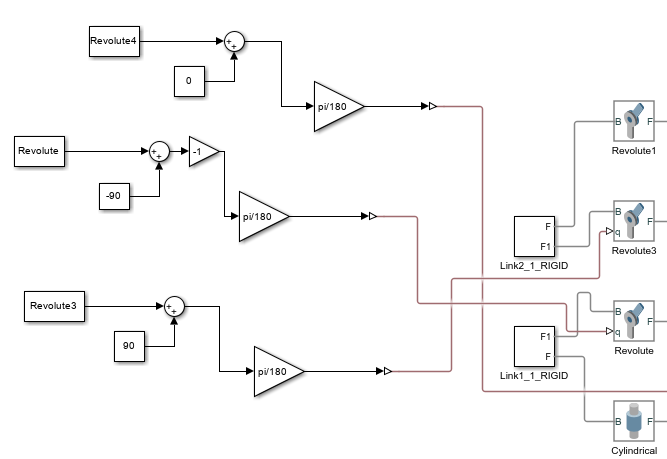
\includegraphics[width=0.5\linewidth]{inputs.PNG}
    \caption{اعمال ورودی به مدل ربات}
    \label{fig:Robot_Input}
\end{figure}

پیش از اعمال ورودی ها به مدل، لازم است زوایای مورد استفاده در کد برنامه نویسی شده با مفاصل ایجاد شده در مدل ربات نگاشت شوند. بنابراین، در مدل استفاده شد از نگاشت های زیر برای تبدیل این زوایا استفاده می کنیم.

\[
\text{Rev4} = \theta_1
\]
\[
\text{Rev} = (\theta_3 - 90^\circ) \cdot (-1)
\]
\[
\text{Rev3} = \theta_2 + 90^\circ
\]

در ادامه، پس از تنظیم موقعیت دستگاه مختصات ربات بر روی ابزار آن و خاموش کردن وضعیت گرانش، مدل را ذخیره می کنیم. بخش انتهایی این مدل، شامل بلوکی برای دریافت مختصات مبدا جهانی و اعمال تبدیل های ناشی از مجموع لینک ها است. در نهایت، خروجی های این بلوک، به صورت R, X, Y, Z به دست می آیند. برای استفاده از این خروجی ها، آنها را به وسیله ی بلوک های To Workspace
به فضای متلب وارد می کنیم.
برای اعمال مقادیر ورودی زوایا به این مدل، با استفاده از کد متلب نوشته شده،مدل را فراخوانی کرده و در نهایت با اجرای کد، می توانیم نتایج را مشاهده کنیم.
در ادامه، به صحت سنجی چهار داده ی ورودی خواهیم پرداخت. برای این کار، مقادیر داده شده به  زوایا ابتدا به وسیله ی ماتریس تبدیل محاسبه شده و سپس نتایج را با نتایج به دست آمده از مدل ربات مقایسه می کنیم.بلوک کلی مورد استفاده در این مدل به صورت زیر می باشد:
\begin{figure}[H]
    \centering
    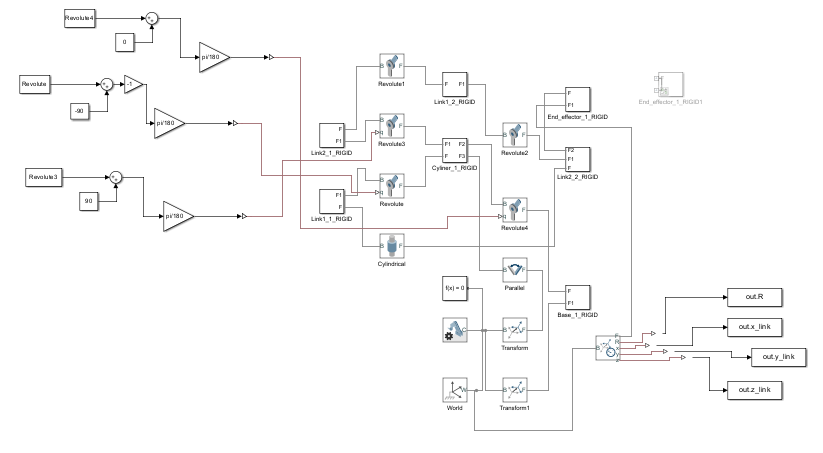
\includegraphics[width=1\linewidth]{simulink.PNG}
    \caption{مدل ربات در SimScape}
    \label{fig:Simulink}
\end{figure}

در این مقایسه، لازم به ذکر است که به دلیل تفاوت تعیین جهت دستگاه های مختصات در دو روش، علامت مقادیر موقعیت و همچنین ماتریس دوران تفاوت هایی در نمایش داند. 
اما مقادیر عددی مطابقت دارند.
\begin{figure}[H]
    \centering
    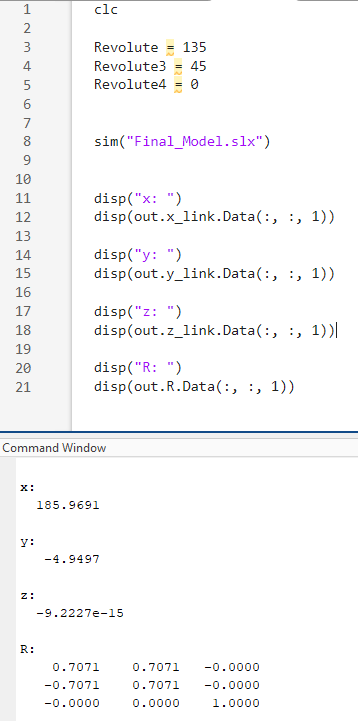
\includegraphics[width=0.5\linewidth]{result1.PNG}
    \caption{نتیجه مدل، آزمایش 1}
    \label{fig:result1}
\end{figure}

\newpage

\begin{figure}[th]
    \centering
    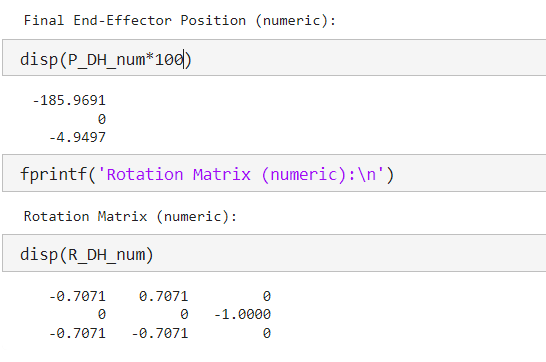
\includegraphics[width=0.5\linewidth]{result1_screen.png}
    \caption{نتیجه کد، آزمایش 1}
    \label{fig:enter-label}
\end{figure}

با بررسی نتیجه ی به دست آمده از این قسمت، می توان مشاهده کرد که محور دوران 
$\theta_1$
در مدل ربات، محور z در نظر گرفته شده است، در حالی که با دستگاه های مختصات مورد استفاده در ماتریس های تبدیل که پیش از این مورد استفاده قرار گرفته اند، این محور y در نظر گرفته شده است.
به همین سبب، ماتریس دوران نیز حول محور های مختلفی لحاظ شده است
همچنین، جهت محور x در راستای مخالف لحاظ شده است و به این دلیل، علامت ان در دو روش متفاوت است.

\begin{figure}[H]
    \centering
    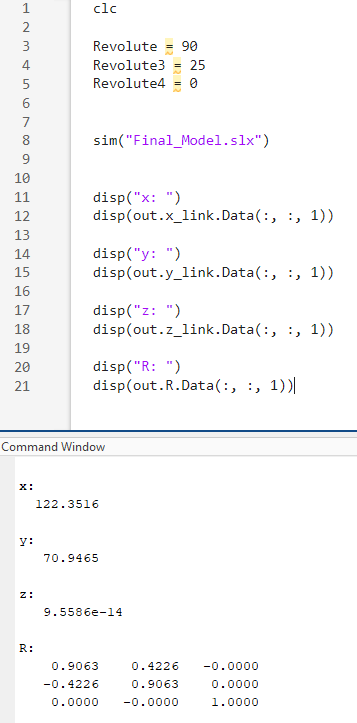
\includegraphics[width=0.5\linewidth]{result2.PNG}
    \caption{نتیجه مدل، آزمایش 2}
    \label{fig:fig:result2}
\end{figure}

\begin{figure}[H]
    \centering
    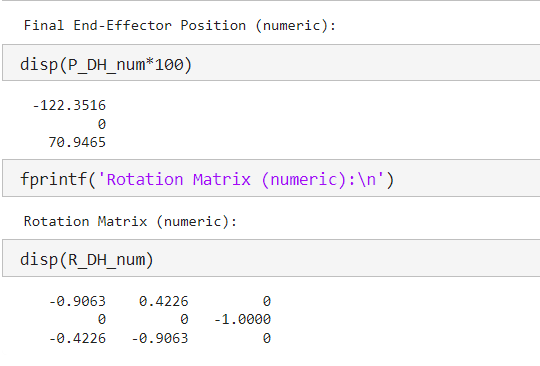
\includegraphics[width=0.5\linewidth]{result2_screen.png}
    \caption{نتیجه کد، آزمایش 2}
    \label{fig:enter-label}
\end{figure}

در این قسمت، مجددا مشاهده می کنیم که مقادیر عددی به دست آمده یکسان هستند، اما به دلیل تفاوت در دستگاه های مختصات که پیش از این توضیح داده شد در نمایش تفاوت دارند.

\begin{figure}[H]
    \centering
    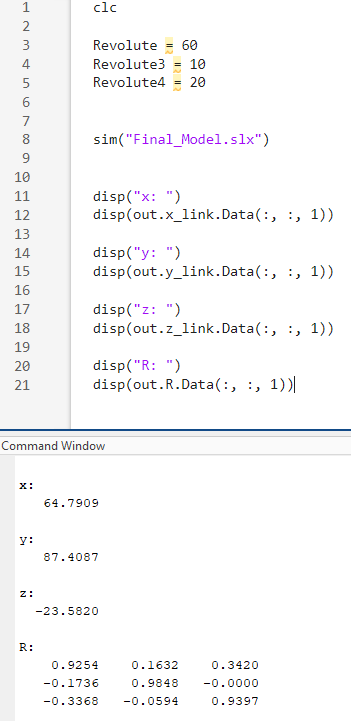
\includegraphics[width=0.5\linewidth]{result4.PNG}
    \caption{نتیجه مدل، آزمایش 3}
    \label{fig:fig:result4}
\end{figure}

\begin{figure}[H]
    \centering
    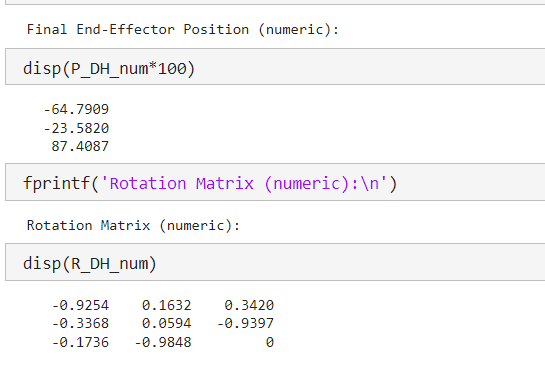
\includegraphics[width=0.5\linewidth]{result4_screen.png}
    \caption{نتیجه کد، آزمایش 3}
    \label{fig:enter-label}
\end{figure}

با آزمایش مدل به دست آمده با زوایای ورودی مختلف، می توانیم نتیجه بگیریم که روش های ارائه شده و مدل طراحی شده عملکرد مناسبی در شبیه سازی عملکرد ربات دارند.

\section{سوال هفتم - فرایند ساخت ربات}
در بخش نهایی از این پروژه، برای ساخت قطعات از طرح های قرار داده شده در پایگاه گیت هاب ذکر شده در فایل سوالات استفاده شده است. طرح های داده شده توسط پرینتر سه بعدی چاپ شده و آماده ی استفاده برای مراحل بعد می باشد. با توجه به زمان بر بودن فرایند چاپ، ویدیو و گزارش های دقیق تر از فرایند ساخت پس از آماده شدن قطعات ارسال خواهد شد.
برای چاپ این قطعات، با در نظر گرفتن استحکام مورد نیاز، از فیلامان با جنس PLA استفاده شده.
همچنین، درصد Fill نیز برای بعضی از قطعات با 40 درصد و برای بعضی دیگر با 50 درصد لحاظ شده است. البته لازم به ذکر است که چهار لایه ی ابتدایی و انتهایی با fill کامل ساخته شده اند.

در این قسمت، تصاویر قطعاتی که برای پرینت آماده هستند نمایش داده شده است. 
\begin{figure}[H]
    \centering
    \begin{minipage}{0.5\linewidth}
        \centering
        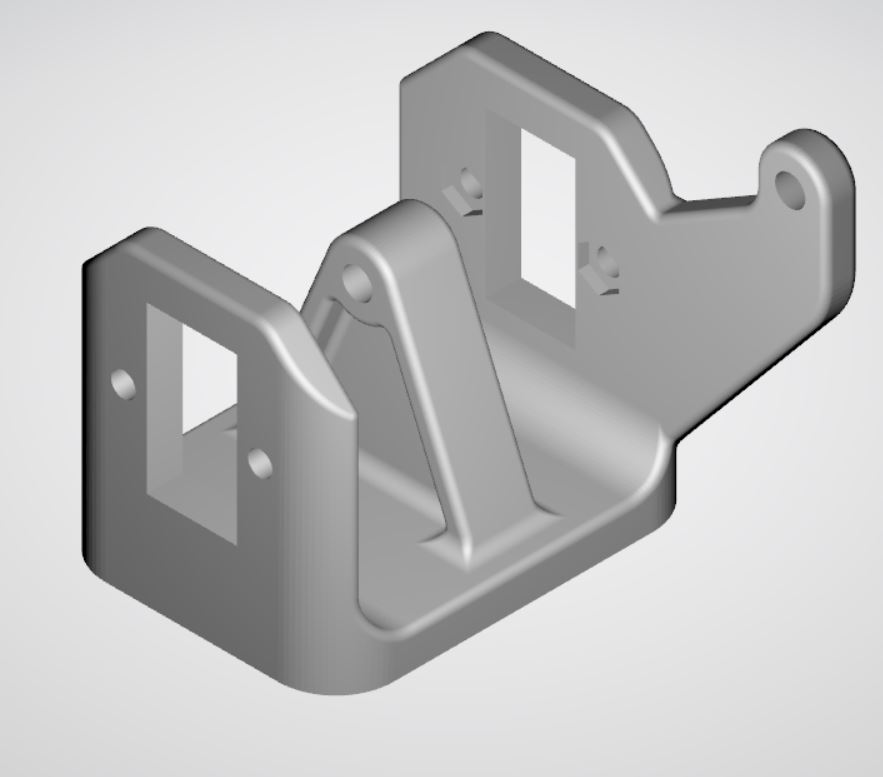
\includegraphics[width=0.9\linewidth]{1.JPG}
        \caption{قطعه 1}
        \label{fig:label1}
    \end{minipage}%
    \begin{minipage}{0.5\linewidth}
        \centering
        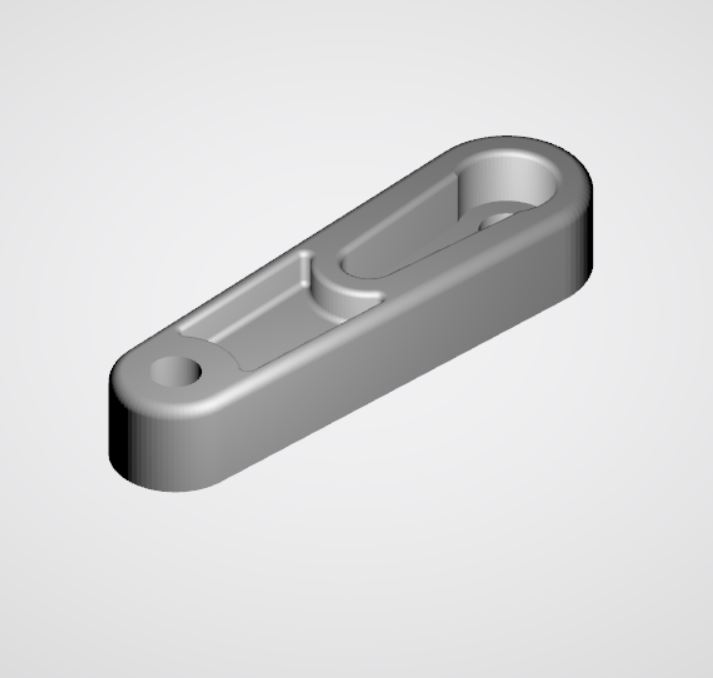
\includegraphics[width=0.9\linewidth]{2.JPG}
        \caption{قطعه 2}
        \label{fig:label2}
    \end{minipage}
\end{figure}

\begin{figure}[H]
    \centering
    \begin{minipage}{0.5\linewidth}
        \centering
        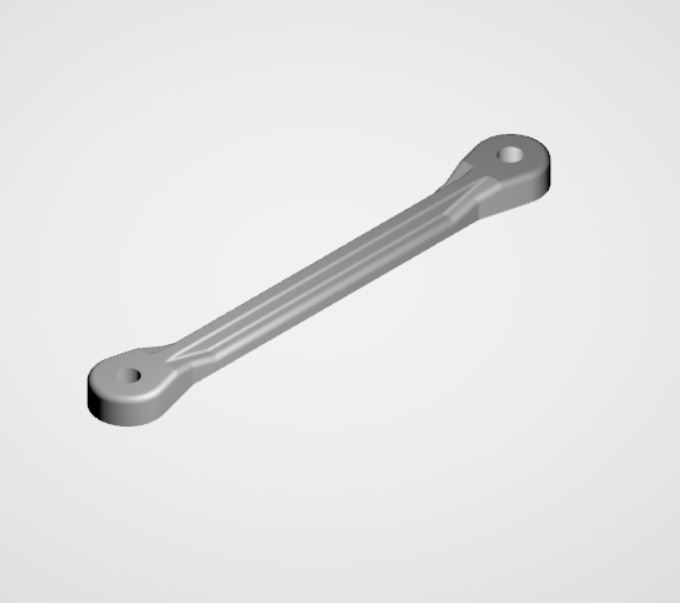
\includegraphics[width=0.9\linewidth]{3.JPG}
        \caption{قطعه 3}
        \label{fig:label3}
    \end{minipage}%
    \begin{minipage}{0.5\linewidth}
        \centering
        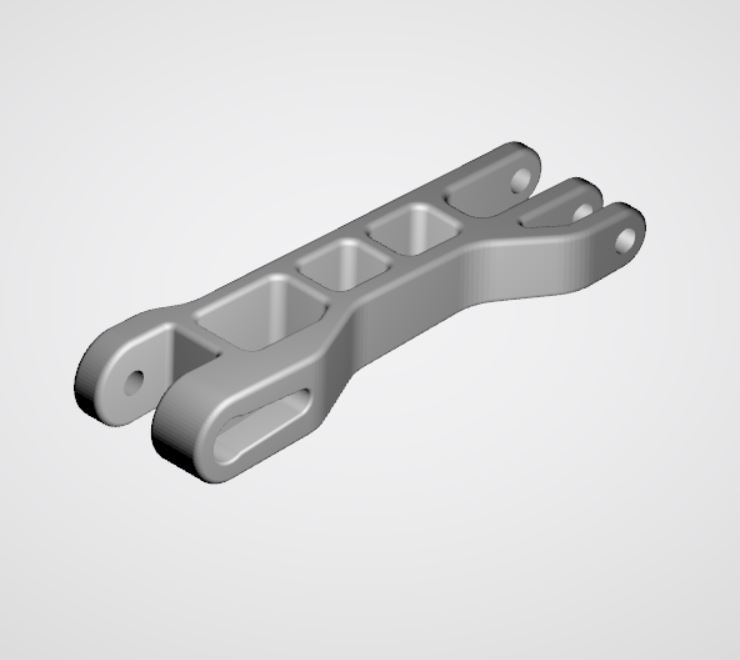
\includegraphics[width=0.9\linewidth]{4.JPG}
        \caption{قطعه 4}
        \label{fig:label4}
    \end{minipage}
\end{figure}

\begin{figure}[H]
    \centering
    \begin{minipage}{0.5\linewidth}
        \centering
        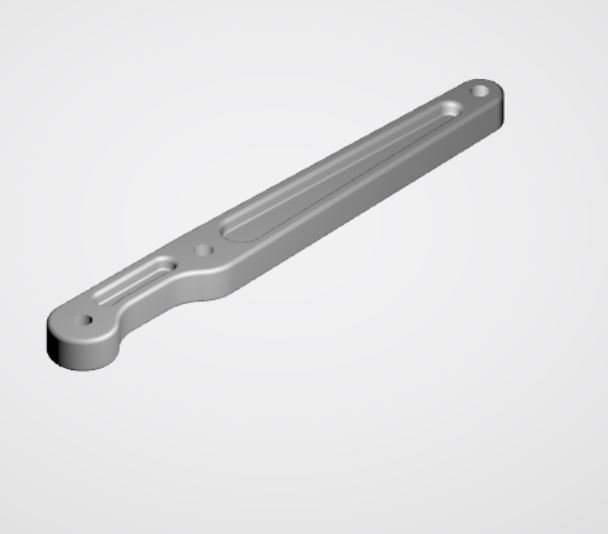
\includegraphics[width=0.9\linewidth]{5.JPG}
        \caption{قطعه 5}
        \label{fig:label5}
    \end{minipage}%
    \begin{minipage}{0.5\linewidth}
        \centering
        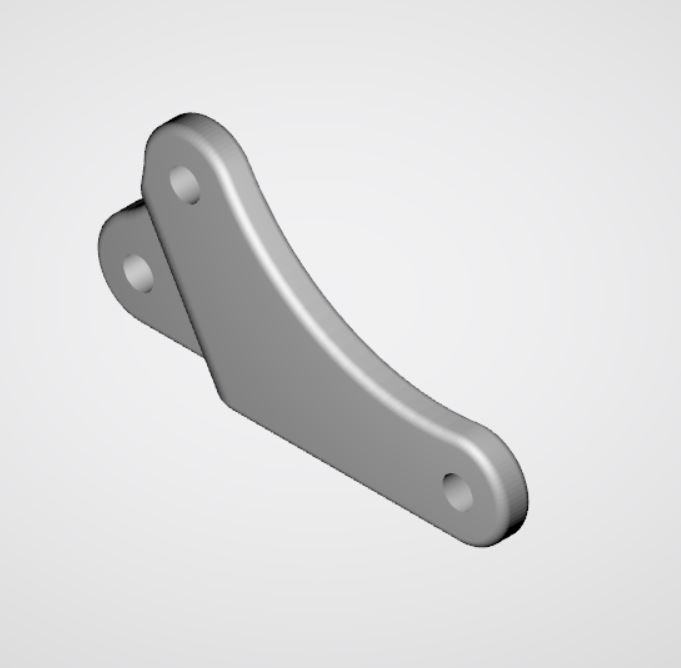
\includegraphics[width=0.9\linewidth]{6.JPG}
        \caption{قطعه 6}
        \label{fig:label6}
    \end{minipage}
\end{figure}

\begin{figure}[H]
    \centering
    \begin{minipage}{0.5\linewidth}
        \centering
        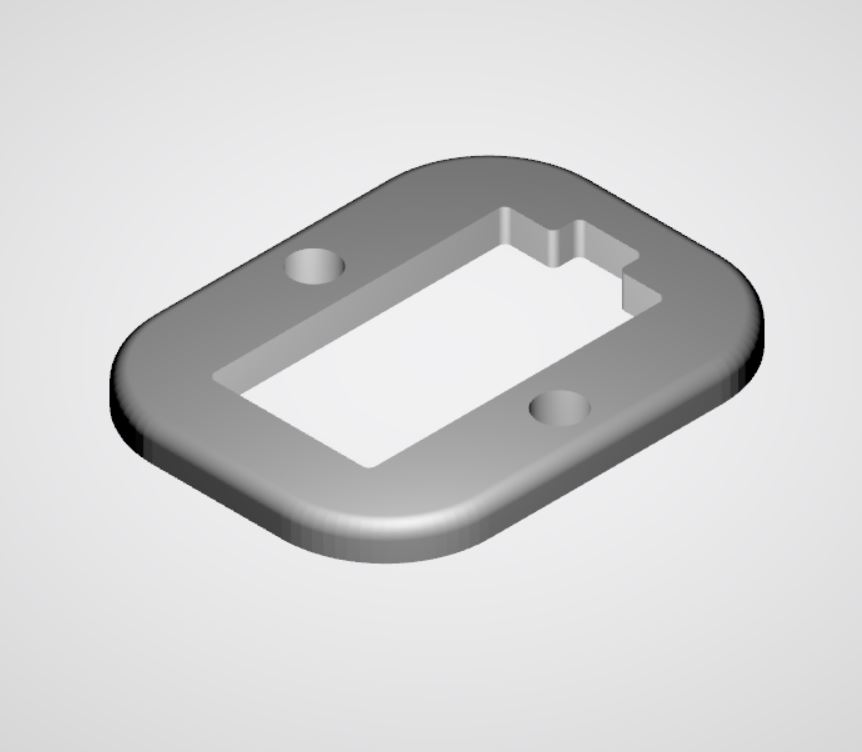
\includegraphics[width=0.9\linewidth]{7.JPG}
        \caption{قطعه 7}
        \label{fig:label7}
    \end{minipage}%
    \begin{minipage}{0.5\linewidth}
        \centering
        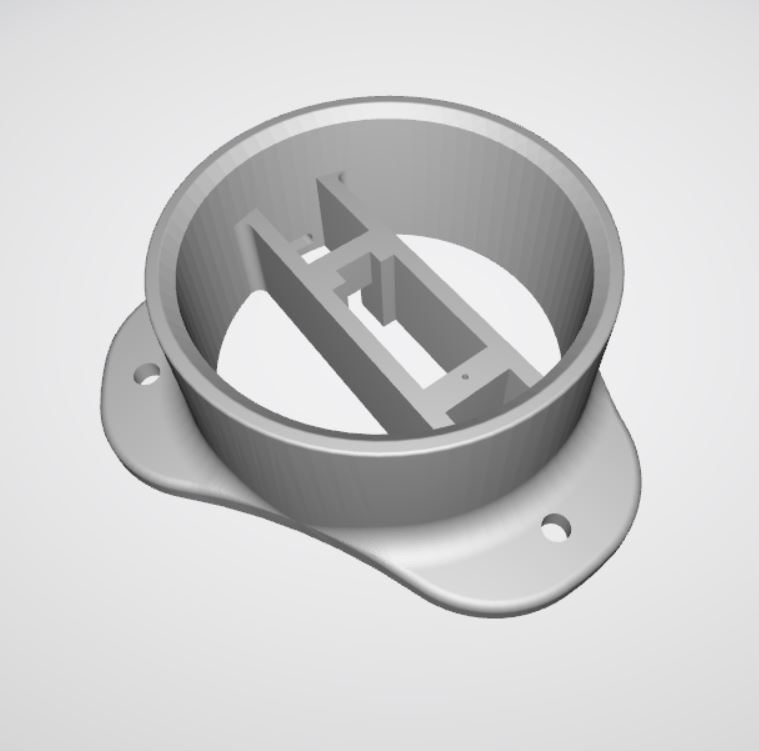
\includegraphics[width=0.9\linewidth]{8.JPG}
        \caption{قطعه 8}
        \label{fig:label8}
    \end{minipage}
\end{figure}

\begin{figure}[H]
    \centering
    \begin{minipage}{0.5\linewidth}
        \centering
        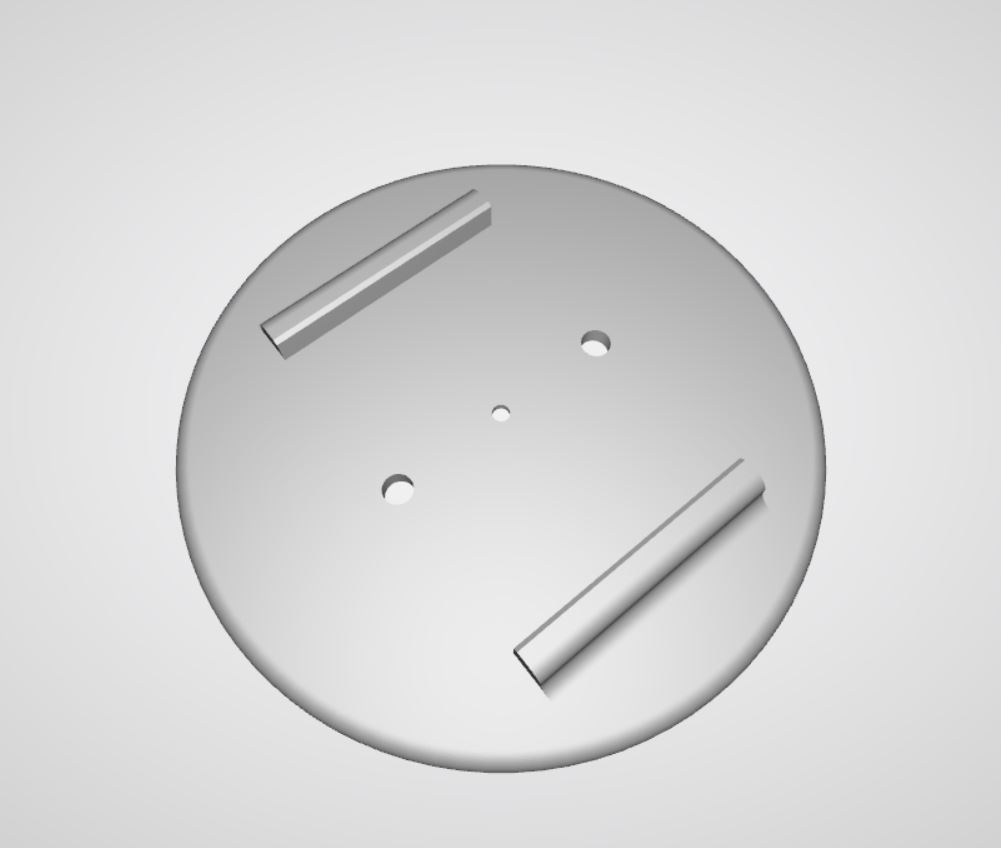
\includegraphics[width=0.9\linewidth]{9.JPG}
        \caption{قطعه 9}
        \label{fig:label9}
    \end{minipage}%
    \begin{minipage}{0.5\linewidth}
        \centering
        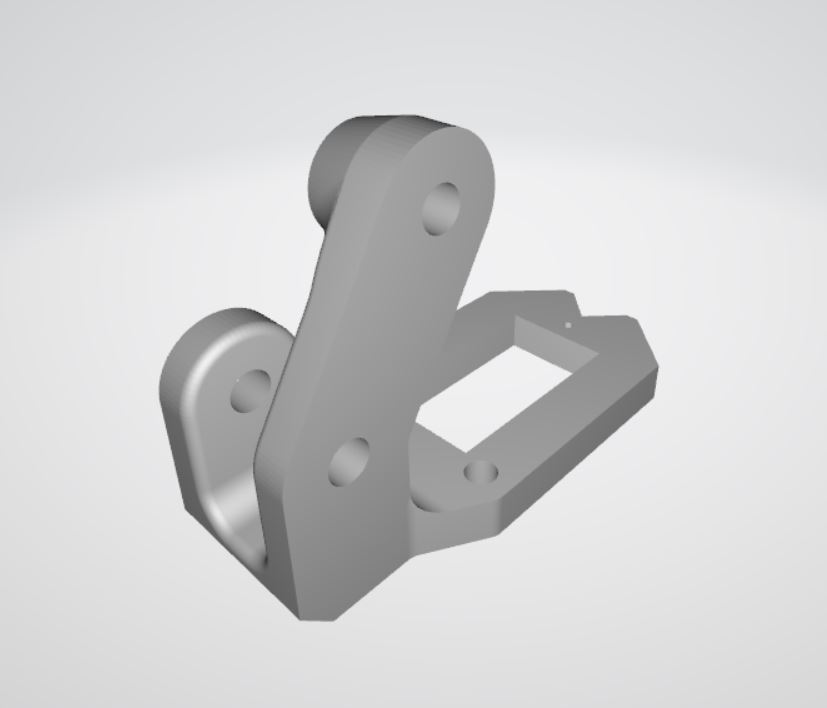
\includegraphics[width=0.9\linewidth]{10.JPG}
        \caption{قطعه 10}
        \label{fig:label10}
    \end{minipage}
\end{figure}
% در این قسمت با نحوه درج برنامه‌ها آشنا می‌شوید:
% \lr{\lstinputlisting[language=Python, caption={My Caption (Python)} \label{Code1}, showstringspaces=false, basicstyle=\ttfamily, backgroundcolor=\color{yellow!15!white}, breaklines=true]{./code/Source.py}}
% \lr{\lstinputlisting[language=MATLAB, caption={My Caption (MATLAB)}, showstringspaces=false, basicstyle=\ttfamily, backgroundcolor=\color{yellow!15!white}, breaklines=true]{./code/Source.m}}
% \lr{\lstinputlisting[language=C++, caption={My Caption (C++)}, showstringspaces=false, basicstyle=\ttfamily, backgroundcolor=\color{yellow!15!white}, breaklines=true]{./code/Source.cpp}}
% \lr{\lstinputlisting[language=C, caption={My Caption (C)}, showstringspaces=false, basicstyle=\ttfamily, backgroundcolor=\color{yellow!15!white}, breaklines=true]{./code/Source.c}}
% \section{عنوان سوال هشتم}
% در این قسمت با نحوۀ ارجاع‌دادن آشنا می‌شوید.
% \subsection{عنوان بخش اول سوال هشتم}
% در این قسمت با نحوۀ ارجاع به سایر منابع آشنا می‌شوید:\\
% \indent
% به صفحۀ درس تشخیص و شناسایی عیب ارجاع داده می‌شود \cite{b1}. 
% به این کتاب‌ها ارجاع داده می‌شود \cite{b2}\cite{b3}.
% برای وارد کردن ارجاع می‌توانید از انتهای فایل 
% \verb|main.tex|
% استفاده کنید و یا با تغییر قالب مرجع‌نویسی،
% به فایل
% \verb|bibliography.bib|
% مراجعه کرده و فرمت
% \verb|.bib|
% را وارد کنید.
% \subsection{عنوان بخش دوم سوال هشتم}
% اگر می‌خواهید به یک شکل، جدول، یا بخش ارجاع دهید می‌توانید به دو صورتی که در ادامه آمده عمل کنید (حالت اول توصیه می‌شود):
% \begin{enumerate}
%     \item \textbf{مورد شماره 1:} \autoref{Section1}, \autoref{eq1}, \autoref{fig1}, \autoref{tab1}, \autoref{Code1}.
%     \item \textbf{مورد شماره 2:} \nameref{Section1}.
% \end{enumerate}
% \subsection{عنوان بخش سوم سوال هشتم}
% اگر می‌خواهید به یک پایگاه اینترنتی ارجاع دهید، می‌توانید از این دستور هم استفاده کنید:
% \href{https://github.com/MJAHMADEE/ARASLaTeXFormats}{گیتهاب (\lr{GitHub})}.

% \section{ضمیمه}
% برای آشنایی بیشتر با \lr{\LaTeX}، با جست‌و‌جو در اینترنت منابع مفیدی خواهید یافت.

%\printbibliography[title=منابع]

% \section*{منابع}

% \renewcommand{\section}[2]{}%
% \begin{thebibliography}{99} % assumes less than 100 references
% %چنانچه مرجع فارسی نیز داشته باشید باید دستور فوق را فعال کنید و مراجع فارسی خود را بعد از این دستور وارد کنید
% \bibitem{b1} \href{https://github.com/MJAHMADEE/MachineLearning2023}{صفحۀ درس یادگیری ماشین.}
% \begin{LTRitems}
% \resetlatinfont
% \bibitem{b2} Steven X. Ding, “Data-driven Design of Fault Diagnosis and Fault-tolerant Control System”, Springer, 2014.
% \bibitem{b3} S. Theodoridis and K. Koutroumbas, "Pattern recognition", Fourth Edition, Academic Press, 2009.
% \end{LTRitems}

% \end{thebibliography}

\end{document}
